\section{Conclusioni} 
\subsection{Considerazioni Finali}
Il lavoro svolto ha portato allo sviluppo di un sistema di sintesi automatica in grado di generare riassunti coerenti a partire da recensioni di cibo. Il sistema è stato progettato per garantire facilità di estensione e adattabilità a diverse tipologie di task, aumentando così la sua versatilità e potenziale applicativo in contesti variegati.\\
Nel corso del progetto sono stati implementati diversi modelli di sintesi automatica, tra cui Seq2SeqLSTM, Seq2SeqBiLSTM, Seq2Seq3BiLSTM, Seq2SeqLSTMGlove e Seq2SeqGRU.
I risultati sono stati valutati attraverso numerose metriche, quali ROUGE, Word Error Rate (WER), Cosine Similarity, BERTScore e \texttt{MyEvaluation}. In particolare,
la BERTScore si è rivelata la metrica più rappresentativa della qualità dei riassunti, in quanto considera il contesto semantico e la similarità delle parole.\\

Inoltre, la metrica \texttt{MyEvaluation} ha fornito una valutazione più dettagliata della qualità dei riassunti, integrando vari fattori e assegnando a ciascuno 
un peso in base alla sua rilevanza. I risultati sperimentali indicano che il modello \textbf{Seq2SeqBiLSTM} ha ottenuto le prestazioni migliori su quasi tutte le metriche, 
suggerendo una superiore capacità di catturare le similarità semantiche tra i riassunti generati e quelli di riferimento.\\

È opportuno sottolineare che i risultati sono stati influenzati dalla scelta del dataset e dalle specifiche caratteristiche dei dati, 
inclusi gli aspetti relativi al preprocessing. Tali elementi evidenziano l'importanza di un'attenta selezione e preparazione dei dati per 
ottimizzare le prestazioni dei modelli di sintesi automatica.

\subsection{Test del Modello Migliore}
Il modello \textbf{Seq2SeqBiLSTM} ha mostrato prestazioni superiori rispetto agli altri modelli implementati.\\
Di seguito vengono riportati alcuni esempi di riassunti generati dal modello \textbf{Seq2SeqBiLSTM} e i rispettivi riassunti di riferimento.\\

\begin{figure}[H]
    \centering
    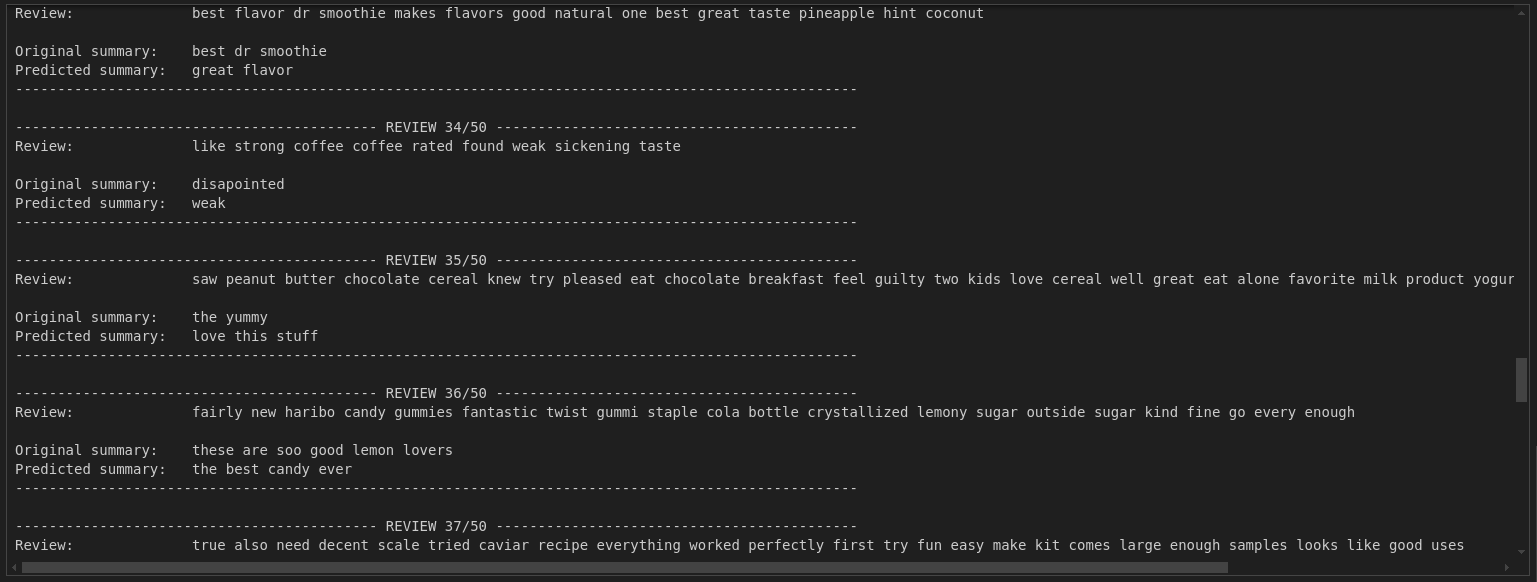
\includegraphics[width=0.75\textwidth]{media/Seq2SeqBiLSTM_inference.png}
    \caption{Esempio di riassunto generato dal modello Seq2SeqBiLSTM}
    \label{fig:example1}
\end{figure}